\subsection{Context}
\begin{frame}\frametitle{Adaptive Systems (ASs)}

\begin{figure}
	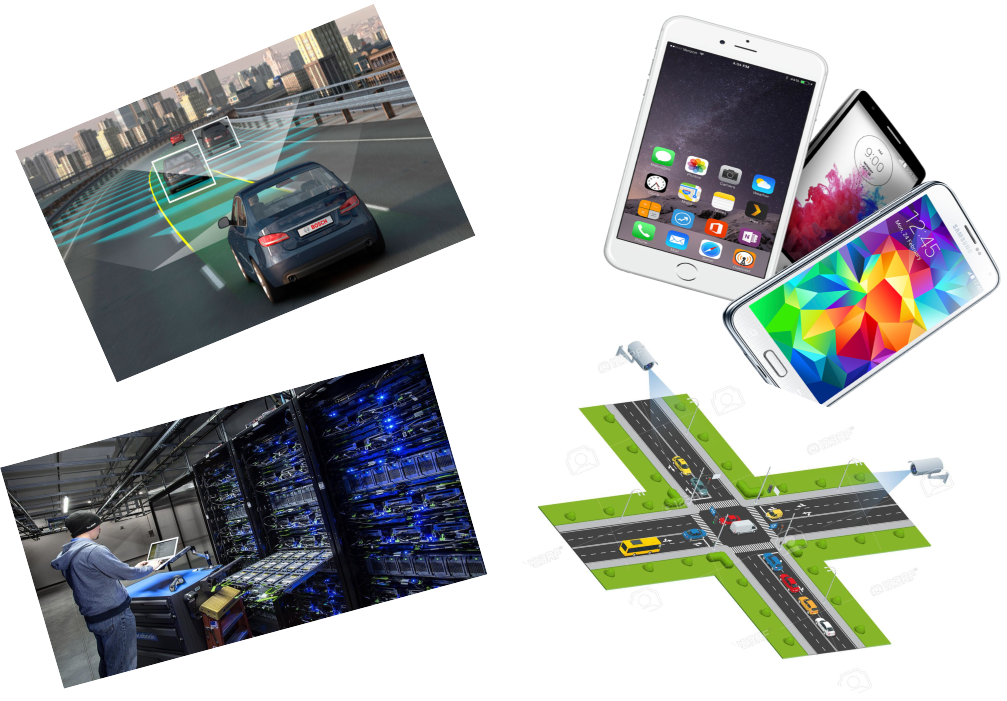
\includegraphics[width=0.8\textwidth]{figures/sas.png}
	\caption{Adaptive Systems are demanded in several domains}
\end{figure}

\end{frame}

\begin{frame}\frametitle{The implementation of ASs}
\begin{figure}
	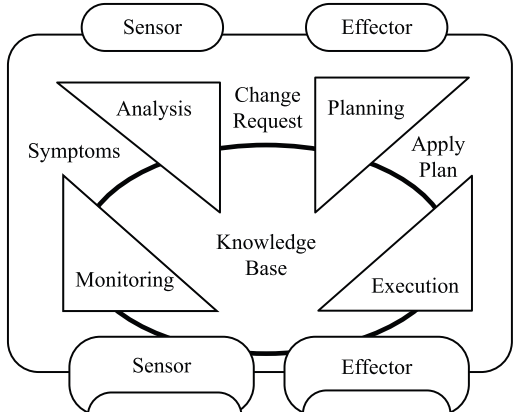
\includegraphics[width=0.7\textwidth]{figures/mapek.png}
	\caption{The autonomic reference model \cite{ibm2005architectural}}
\end{figure}

\end{frame}

\begin{frame}\frametitle{The implementation of ASs}

\textit{``Something in architecture design and its implementation is no longer adequate.''} \cite{Zimmermann2017}

\begin{figure}
	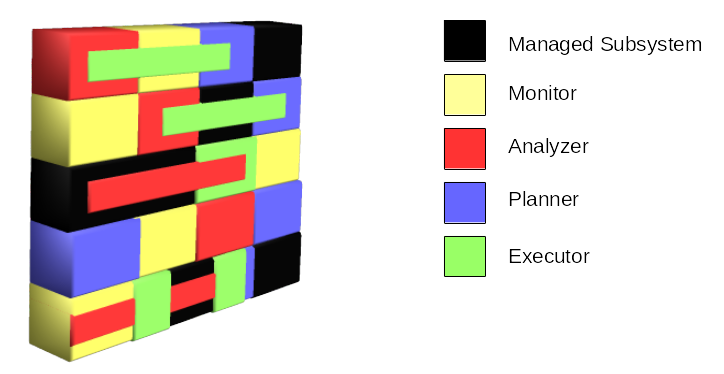
\includegraphics[width=0.8\textwidth]{figures/concern.png}
	\caption{AS abstractions are not evident in source code}
\end{figure}

\end{frame}

\begin{frame}\frametitle{Motivations}

\begin{itemize}
	\item Software engineers do not follow architectural models of ASs;
	\vspace{0.5cm}
	\item The lack of architectural smells catalogs of ASs;
	\vspace{0.5cm}
	\item The lack of approaches for identifying architectural smells of ASs.
\end{itemize}

\end{frame}
\subsection{Objectives}
\begin{frame}\frametitle{Objectives}

\begin{block}{Objective I}
	Characterizing architectural smells in the context of ASs.

\end{block}
\vspace{0.5cm}
\pause
\begin{block}{Objective II}
	Identifying a set of architectural smells of ASs. 
\end{block}
\vspace{0.5cm}
\pause

\begin{block}{Objective III}
	Supporting software engineers on the identification of architectural smells of ASs.
\end{block}


\end{frame}

\subsection{Contributions}
\begin{frame}\frametitle{Contributions}


\tikzstyle{q} = [rectangle, draw, fill=RoyalBlue, node distance=2cm, text width=12em,  text=white, rounded corners, minimum height=3em, thick]

\tikzstyle{r} = [rectangle, draw, fill=green!50!black, node distance=2cm, text width=12em,  text=white, rounded corners, minimum height=3em, minimum width=6em, thick]

\tikzstyle{v} = [rectangle, draw, fill=white, node distance=2cm, text width=10em, text centered,  rounded corners, minimum height=3em, minimum width=10em, thick]

\tikzstyle{l} = [draw, -latex',thick]

\begin{tikzpicture}
\node[q] (g1) at (0,0) {\textbf{Objective 1:}\\	{\scriptsize \textbf{Characterizing architectural smells in the context of ASs}}};
\node [q, below = 0.5cm of g1] (g2) {\textbf{Objective 2:}\\	{\scriptsize \textbf{Identifying a set of architectural smells of ASs}}};
\node [q, below = 0.5cm of g2] (g3) {\textbf{Objective 3:}\\	{\scriptsize \textbf{Supporting software engineers on the identification of architectural smells of ASs}}};


\node [r, right= 0.5cm of g1] (c1) {\textbf{Contribution 1:} \\ {\scriptsize \textbf{A catalog with formal and informal specifications}}};
\node [r, right= 0.5cm of g2] (c2) {\textbf{Contribution 2:} \\ {\scriptsize \textbf{A set of rules for applying on the identification of the smells}}};
\node [r, right= 0.5cm of g3] (c3) {\textbf{Contribution 3:} \\ {\scriptsize \textbf{A semi-automated tool for applying the identification rules}}};


\path [l] (g1) -- (c1);
\path [l] (g2) --  (c2);
\path [l] (g3) --  (c3);


\end{tikzpicture}


\end{frame}

